For a particular amplifier connected in a feedback loop in which the output voltage is sampled,measurement of the output resistance before and after the loop is connected shows a change by a factor of 100.Is the resistance with feedback higher or lower?What is the value of the loop gain GH? If $R_{of}$ is 100 $\Omega$ ,what is $R_o$ without feedback.
\begin{enumerate}[label=\arabic*.,ref=\theenumi]

\numberwithin{equation}{enumi}
\numberwithin{figure}{enumi}

\item Find the loop gain $GH$.
\\
\solution
We know that,
\begin{align}
    R_o = R_{of}(1+GH)
    \label{eq:ee18btech11042_1}
\end{align}
Output resistance before and after the loop is connected changes bya factor 100.So,

\begin{align}
    GH =99
\end{align}
Open loop gain GH is  99.
\newline
Given,
\begin{align}
    R_{of} = 100 
    \label{eq:ee18btech11042_3}
\end{align}
\begin{align}
    R_o = 100(1+99)
    \label{eq:ee18btech11042_4}
\end{align}
\begin{align}
    R_o = 10000
    \label{eq:ee18btech11042_5}
\end{align}
Output resistance without feedback  is   10k$\Omega$
\newline
Output resistance without feedback is greater than with feedback.
\item
The following code generates the values
\begin{lstlisting}
codes/ee18btech11042.py
\end{lstlisting}

\item Design a circuit.
\solution


\begin{figure}[!h]
		\resizebox{\columnwidth}{!}{\begin{circuitikz}[american]


    \ctikzset{tripoles/mos style/arrows}
    \draw(0,0)to [resistor, l = $R_S$] (1,0)--(3,0);
    \draw(3,0)--(4,0)--(4,-0.5) to [resistor, l = $R_{id}$,v> = $V_1$](4,-1.5)--(4,-2.5);
    
    \draw(4,-2.5)--(1,-2.5)--(1,-4)--(1,-8)--(1,-9)to [resistor,l = $R_1$] (1,-10);
    \draw(1,-10) node[ground]{};
    \draw(0,0)--(-2,0) to [V,l = $V_s$] (-2,-4);
    \draw(-2,-4) node[ground]{};
    \draw(1,-8)--(3,-8) to [resistor,l = $R_2$] (5,-8)-- (9,-8)--(9,-1.5);
    \draw(9,-1.5)--(10,-1.5)--(10,-2) to [resistor,l = $R_L$](10,-3) --(10,-4);
    \draw(10,-4)node[ground]{};
    \draw(4,-1.5) to [open,](7,-1.5);
    \draw(7,-1.5)--(7.5,-1.5) to [resistor,l = $r_o$](8.5,-1.5);
    \draw(8.5,-1.5)--(9,-1.5);
    \draw(7,-1.5)--(7,-2) to [cV,l = $\mu V_1$](7,-2.75)--(7,-3.25);
    \draw (7,-3.25)node[ground]{};
    \draw(8.75,-1.5)--(3,-5.75)--(3,1.5)--(8.75,-1.5);
    \draw(10,-1.5) node[circle,fill,inner sep = 2pt ,label = right:$V_o$]{};
    \end{circuitikz}}
\caption{Amplifier Circuit}
\label{fig:ee18btech11042_1}
\end{figure}
Feedback Gain
\begin{align}
    H = \frac{R_1}{R_1+R_2} = \frac{1}{40}
    \label{eq:ee18btech11042_6}
\end{align}
\begin{figure}[!h]
		\resizebox{\columnwidth}{!}{\begin{circuitikz}[american]
    
    \ctikzset{tripoles/mos style/arrows}
    \draw(0,0) to [resistor,l = $R_s$] (2,0) --(3,0)--(3,-1) to [resistor,l = $R_{id}$,v>=$V_1$](3,-3);
    \draw (3,-3) to [resistor,l = $R_1//R_2$] (0,-3);
    \draw(0,0) to [open,v>=$V_f$](0,-3);
    \draw(3,0) to [open] (4,0);
    \draw (4,0)--(5,0) to [resistor,l = $ r_o$] (6,0)--(6.5,0);
    \draw(6.5,0) to [resistor,l = $R_1+R_2$](6.5,-3);
    \draw(6.5,-3) node [ground]{};
    \draw(6.5,0)--(8.5,0)to [resistor,l = $R_L$] (8.5,-3);
    \draw(8.5,-3)node [ground]{};
    \draw(4,0)to [cV,l = $\mu V_1$] (4,-3);
    \draw(4,-3) node[ground]{};
    \draw(8.5,0)node[circle,fill,inner sep = 2pt,label = $V_o$]{};
    \end{circuitikz}
 }
\caption{H circuit}
\label{fig:ee18btech11042_2}
\end{figure}
From fig \ref{fig:ee18btech11042_2},
Open Loop  input resistance
\begin{align}
    R_{in} = R_s+R_{id}+(R_1//R_2)
    \label{eq:ee18btech11042_7}
\end{align}
Open loop output resistance 
\begin{align}
    R_o = r_o//R_L//(R_1+R_2)
    \label{eq:ee18btech11042_8}
\end{align}
Open Loop gain
\begin{align}
    G = \mu \frac{R_{id}}{R_s+R_{id}+(R_1//R_2)}\frac{R_L//R_1+R_2}{(r_o+(R_L//R_1+R_2))}
    \label{eq:ee18btech11042_9}
\end{align}
\begin{table}[!h]
    \centering
  	\resizebox{\columnwidth}{!}{%%%%%%%%%%%%%%%%%%%%%%%%%%%%%%%%%%%%%%%%%%%%%%%%%%%%%%%%%%%%%%%%%%%%%%
%%                                                                  %%
%%  This is the header of a LaTeX2e file exported from Gnumeric.    %%
%%                                                                  %%
%%  This file can be compiled as it stands or included in another   %%
%%  LaTeX document. The table is based on the longtable package so  %%
%%  the longtable options (headers, footers...) can be set in the   %%
%%  preamble section below (see PRAMBLE).                           %%
%%                                                                  %%
%%  To include the file in another, the following two lines must be %%
%%  in the including file:                                          %%
%%        \def\inputGnumericTable{}                                 %%
%%  at the beginning of the file and:                               %%
%%        \input{name-of-this-file.tex}                             %%
%%  where the table is to be placed. Note also that the including   %%
%%  file must use the following packages for the table to be        %%
%%  rendered correctly:                                             %%
%%    \usepackage[latin1]{inputenc}                                 %%
%%    \usepackage{color}                                            %%
%%    \usepackage{array}                                            %%
%%    \usepackage{longtable}                                        %%
%%    \usepackage{calc}                                             %%
%%    \usepackage{multirow}                                         %%
%%    \usepackage{hhline}                                           %%
%%    \usepackage{ifthen}                                           %%
%%  optionally (for landscape tables embedded in another document): %%
%%    \usepackage{lscape}                                           %%
%%                                                                  %%
%%%%%%%%%%%%%%%%%%%%%%%%%%%%%%%%%%%%%%%%%%%%%%%%%%%%%%%%%%%%%%%%%%%%%%



%%  This section checks if we are begin input into another file or  %%
%%  the file will be compiled alone. First use a macro taken from   %%
%%  the TeXbook ex 7.7 (suggestion of Han-Wen Nienhuys).            %%
\def\ifundefined#1{\expandafter\ifx\csname#1\endcsname\relax}


%%  Check for the \def token for inputed files. If it is not        %%
%%  defined, the file will be processed as a standalone and the     %%
%%  preamble will be used.                                          %%
\ifundefined{inputGnumericTable}

%%  We must be able to close or not the document at the end.        %%
	\def\gnumericTableEnd{\end{document}}


%%%%%%%%%%%%%%%%%%%%%%%%%%%%%%%%%%%%%%%%%%%%%%%%%%%%%%%%%%%%%%%%%%%%%%
%%                                                                  %%
%%  This is the PREAMBLE. Change these values to get the right      %%
%%  paper size and other niceties.                                  %%
%%                                                                  %%
%%%%%%%%%%%%%%%%%%%%%%%%%%%%%%%%%%%%%%%%%%%%%%%%%%%%%%%%%%%%%%%%%%%%%%

	\documentclass[12pt%
			  %,landscape%
                    ]{report}
       \usepackage[latin1]{inputenc}
       \usepackage{fullpage}
       \usepackage{color}
       \usepackage{array}
       \usepackage{longtable}
       \usepackage{calc}
       \usepackage{multirow}
       \usepackage{hhline}
       \usepackage{ifthen}

	\begin{document}


%%  End of the preamble for the standalone. The next section is for %%
%%  documents which are included into other LaTeX2e files.          %%
\else

%%  We are not a stand alone document. For a regular table, we will %%
%%  have no preamble and only define the closing to mean nothing.   %%
    \def\gnumericTableEnd{}

%%  If we want landscape mode in an embedded document, comment out  %%
%%  the line above and uncomment the two below. The table will      %%
%%  begin on a new page and run in landscape mode.                  %%
%       \def\gnumericTableEnd{\end{landscape}}
%       \begin{landscape}


%%  End of the else clause for this file being \input.              %%
\fi

%%%%%%%%%%%%%%%%%%%%%%%%%%%%%%%%%%%%%%%%%%%%%%%%%%%%%%%%%%%%%%%%%%%%%%
%%                                                                  %%
%%  The rest is the gnumeric table, except for the closing          %%
%%  statement. Changes below will alter the table's appearance.     %%
%%                                                                  %%
%%%%%%%%%%%%%%%%%%%%%%%%%%%%%%%%%%%%%%%%%%%%%%%%%%%%%%%%%%%%%%%%%%%%%%

\providecommand{\gnumericmathit}[1]{#1} 
%%  Uncomment the next line if you would like your numbers to be in %%
%%  italics if they are italizised in the gnumeric table.           %%
%\renewcommand{\gnumericmathit}[1]{\mathit{#1}}
\providecommand{\gnumericPB}[1]%
{\let\gnumericTemp=\\#1\let\\=\gnumericTemp\hspace{0pt}}
 \ifundefined{gnumericTableWidthDefined}
        \newlength{\gnumericTableWidth}
        \newlength{\gnumericTableWidthComplete}
        \newlength{\gnumericMultiRowLength}
        \global\def\gnumericTableWidthDefined{}
 \fi
%% The following setting protects this code from babel shorthands.  %%
 \ifthenelse{\isundefined{\languageshorthands}}{}{\languageshorthands{english}}
%%  The default table format retains the relative column widths of  %%
%%  gnumeric. They can easily be changed to c, r or l. In that case %%
%%  you may want to comment out the next line and uncomment the one %%
%%  thereafter                                                      %%
\providecommand\gnumbox{\makebox[0pt]}
%%\providecommand\gnumbox[1][]{\makebox}

%% to adjust positions in multirow situations                       %%
\setlength{\bigstrutjot}{\jot}
\setlength{\extrarowheight}{\doublerulesep}

%%  The \setlongtables command keeps column widths the same across  %%
%%  pages. Simply comment out next line for varying column widths.  %%
\setlongtables

\setlength\gnumericTableWidth{%
	100pt+%
	100pt+%
0pt}
\def\gumericNumCols{2}
\setlength\gnumericTableWidthComplete{\gnumericTableWidth+%
         \tabcolsep*\gumericNumCols*2+\arrayrulewidth*\gumericNumCols}
\ifthenelse{\lengthtest{\gnumericTableWidthComplete > \linewidth}}%
         {\def\gnumericScale{\ratio{\linewidth-%
                        \tabcolsep*\gumericNumCols*2-%
                        \arrayrulewidth*\gumericNumCols}%
{\gnumericTableWidth}}}%
{\def\gnumericScale{1}}

%%%%%%%%%%%%%%%%%%%%%%%%%%%%%%%%%%%%%%%%%%%%%%%%%%%%%%%%%%%%%%%%%%%%%%
%%                                                                  %%
%% The following are the widths of the various columns. We are      %%
%% defining them here because then they are easier to change.       %%
%% Depending on the cell formats we may use them more than once.    %%
%%                                                                  %%
%%%%%%%%%%%%%%%%%%%%%%%%%%%%%%%%%%%%%%%%%%%%%%%%%%%%%%%%%%%%%%%%%%%%%%

\ifthenelse{\isundefined{\gnumericColA}}{\newlength{\gnumericColA}}{}\settowidth{\gnumericColA}{\begin{tabular}{@{}p{75pt*\gnumericScale}@{}}x\end{tabular}}
\ifthenelse{\isundefined{\gnumericColB}}{\newlength{\gnumericColB}}{}\settowidth{\gnumericColB}{\begin{tabular}{@{}p{90pt*\gnumericScale}@{}}x\end{tabular}}

\begin{tabular}[c]{%
	b{\gnumericColA}%
	b{\gnumericColB}%
	}

%%%%%%%%%%%%%%%%%%%%%%%%%%%%%%%%%%%%%%%%%%%%%%%%%%%%%%%%%%%%%%%%%%%%%%
%%  The longtable options. (Caption, headers... see Goosens, p.124) %%
%	\caption{The Table Caption.}             \\	%
% \hline	% Across the top of the table.
%%  The rest of these options are table rows which are placed on    %%
%%  the first, last or every page. Use \multicolumn if you want.    %%

%%  Header for the first page.                                      %%
%	\multicolumn{3}{c}{The First Header} \\ \hline 
%	\multicolumn{1}{c}{colTag}	%Column 1
%	&\multicolumn{1}{c}{colTag}	%Column 2
%	&\multicolumn{1}{c}{colTag}	\\ \hline %Last column
%	\endfirsthead

%%  The running header definition.                                  %%
%	\hline
%	\multicolumn{3}{l}{\ldots\small\slshape continued} \\ \hline
%	\multicolumn{1}{c}{colTag}	%Column 1
%	&\multicolumn{1}{c}{colTag}	%Column 2
%	&\multicolumn{1}{c}{colTag}	\\ \hline %Last column
%	\endhead

%%  The running footer definition.                                  %%
%	\hline
%	\multicolumn{3}{r}{\small\slshape continued\ldots} \\
%	\endfoot

%%  The ending footer definition.                                   %%
%	\multicolumn{3}{c}{That's all folks} \\ \hline 
%	\endlastfoot
%%%%%%%%%%%%%%%%%%%%%%%%%%%%%%%%%%%%%%%%%%%%%%%%%%%%%%%%%%%%%%%%%%%%%%

\hhline{|-|-}
	 \multicolumn{1}{|p{\gnumericColA}|}%
	{\gnumericPB{\centering}$G$}
	&\multicolumn{1}{p{\gnumericColB}|}%
	{\gnumericPB{\centering}$g_{m}R_{D}$}
	
\\
\hhline{|--|}
	 \multicolumn{1}{|p{\gnumericColA}|}%
	{\gnumericPB{\centering}$H$}
	&\multicolumn{1}{p{\gnumericColB}|}%
	{\gnumericPB{\centering}$\cfrac{R_{1}}{R_{1}+R_{2}}$}
\\
\hhline{|--|}
	 \multicolumn{1}{|p{\gnumericColA}|}%
	{\gnumericPB{\centering}$R_{i}$}
	&\multicolumn{1}{p{\gnumericColB}|}%
	{\gnumericPB{\centering}$\cfrac{1}{g_{m}}$}
\\
\hhline{|--|}
	 \multicolumn{1}{|p{\gnumericColA}|}%
	{\gnumericPB{\centering}$R_{o}$}
	&\multicolumn{1}{p{\gnumericColB}|}%
	{\gnumericPB{\centering}$R_{D}$}
\\
\hhline{|--|}
	 \multicolumn{1}{|p{\gnumericColA}|}%
	{\gnumericPB{\centering}$R_{if}$}
	&\multicolumn{1}{p{\gnumericColB}|}%
	{\gnumericPB{\centering}$(\cfrac{1}{g_{m}})(1 + \cfrac{g_{m}R_{D}R_{1}}{R_{1}+R_{2}})$}
\\
\hhline{|--|}
	 \multicolumn{1}{|p{\gnumericColA}|}%
	{\gnumericPB{\centering}$R_{of}$}
	&\multicolumn{1}{p{\gnumericColB}|}%
	{\gnumericPB{\centering}$\cfrac{R_{D}}{1 + \cfrac{g_{m}R_{D}R_{1}}{R_{1}+R_{2}}}$}
\\
\hhline{|-|-}
\end{tabular}

\ifthenelse{\isundefined{\languageshorthands}}{}{\languageshorthands{\languagename}}
\gnumericTableEnd}
    \caption{parameter values}
    \label{table:ee18btech11042_1}
\end{table}

 Closed Loop Gain   $\frac{G}{1+GH}$  is 39.6


\item Verify through spice.
\newline
The following file provides how to simulate the spice file.
\begin{lstlisting}
spice/ee18btech11042/readme
\end{lstlisting}


 The following is .net list file for spice simulation
 
\begin{lstlisting}
spice/ee18btech11042/ee18btech11042.net
\end{lstlisting}
Given,
\begin{align}
    V_s (t)= sin(2000\pi t)
    \label{eq:ee18btech11042_11}
\end{align}
We got output as
\begin{align}
    V_o(t) = 40 sin(2000\pi t)
    \label{eq:ee18btech11042_12}
\end{align}
Overall gain  $\frac{V_o(t)}{V_{in}(t)}$ is 40 same as thereotical value.
\begin{figure}[!ht]
    
    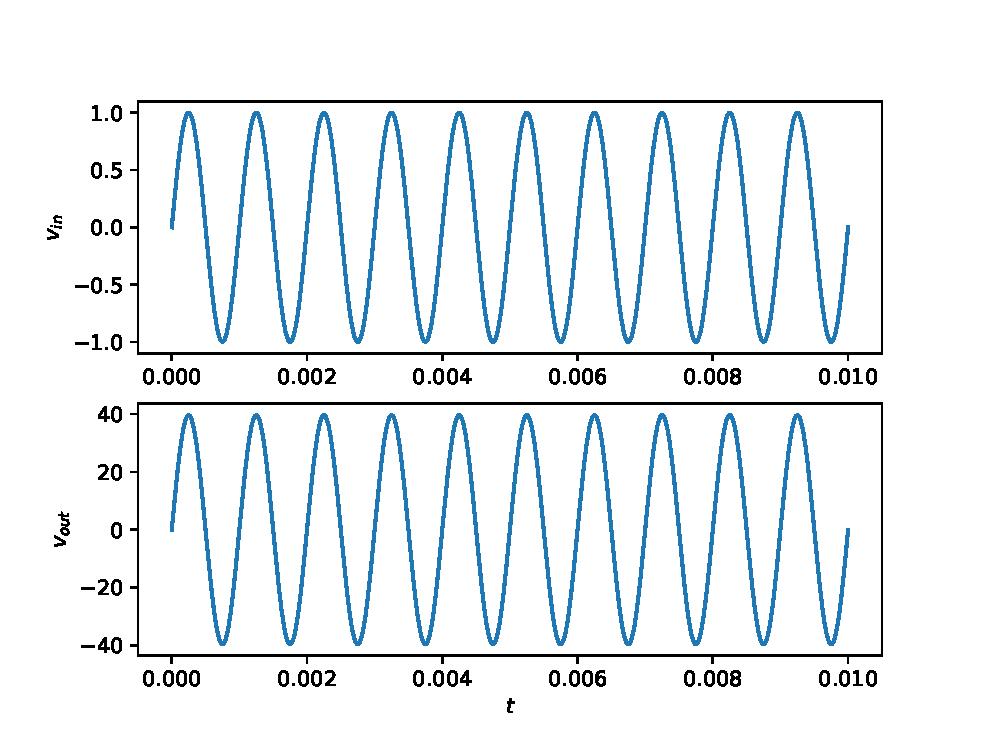
\includegraphics[width = \columnwidth]{./spice/ee18btech11042/spice.eps}
    \caption{Time response of system}
    \label{fig:ee18btech11042_3}
\end{figure}
The following code creates the python plots.
\begin{lstlisting}
spice/ee18btech11042/ee18btech11042_spice.py
\end{lstlisting}







\end{enumerate}



